%%
%% Dibbler - a portable DHCPv6
%%
%% authors: Tomasz Mrugalski <thomson@klub.com.pl>
%%
%% released under GNU GPL v2 licence
%%
%%

\section{Intro}
First of all, as an author I would like to thank you for your interest
in this DHCPv6 implementation. If this documentation doesn't answer
your questions or you have any suggestions, feel free to contact
me as explained in \hyperlink{contact}{Contact} section. Also be sure
to check out Dibbler website: \url{http://klub.com.pl/dhcpv6/}.

\begin{flushright}
\emph{Tomasz Mrugalski}
\end{flushright}

\subsection{Overview}

\emph{Dynamic Host Configuration Protocol for IPv6}, often abbreviated
as DHCPv6, is a protocol, which is used to automatically configure IPv6
capable computers and other equipment located in a local network. This
protocol defines \emph{clients} (i.e. nodes, which want to be configured),
\emph{servers} (i.e. nodes, which provide configuration to clients) and
\emph{relays} (i.e. nodes, which are connected to more than one network and
are able to forward traffic between local clients and remote
servers). Also, special type of DHCPv6 entity called \emph{requestor}
has been defined. It is used by network administrator to query servers
about their status and assigned parameters.

Dibbler is a portable DHCPv6 solution, which features server, client and
relay. Currently there are ports available for many Windows platforms
ranging from NT4 to Windows 8, Linux 2.4 or later systems and Mac OS
(experimental). See Section \ref{requirements} for details. It supports both stateful
(i.e. IPv6 address granting) and stateless (i.e. options granting)
autoconfiguration. Besides basic
functionality (specified in basic DHCPv6 spec, RFC3315 \cite{rfc3315}),
it also offers serveral enhancements, e.g. DNS servers and domain names
configuration.

Dibbler is an open source software, distributed under
\href{http://www.gnu.org/copyleft/gpl.html}{GNU GPL} v2 licence. It means
that it is freely available, free of charge and can be used by anyone
(including commercial users). Source code is also provided, so anyone
skilled enough can fix bugs, add new features and distribute his/her
own version.

\emph{Requestor} support has been added in version 0.7.0RC1. Requestor
is a separate entity, which sends queries to the server regarding
leases to specific clients. It is possible to ask a server, who has
specific address or what addresses are assigned to a specific client.
This feature is part of the lease query mechanism defined in
\cite{rfc5007} and is considered advanced topic. If you don't know
what lease query is, you definetely don't need it.

\begin{figure}[ht]
\begin{center}
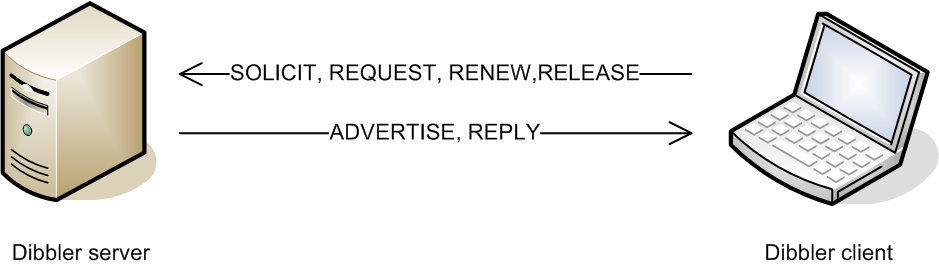
\includegraphics[width=0.7\textwidth]{dibbler-srv-cli}
\caption{\emph{General DHCPv6 operation}}
\end{center}
\end{figure}

Dibbler 1.0.0RC1 supports all features specified in RFC3315. In
particular the following features are supported:
\begin{itemize}
\item Basic server discovery and address assignment (\msg{SOLICIT},
      \msg{ADVERTISE}, \msg{REQUEST} and \msg{REPLY} messages) -- This
      is a most common case: client discovers servers available in the
      local network, then asks for an address (and possibly additional
      options like DNS configuration), which is granted by a~server.

\begin{figure}[ht]
\begin{center}
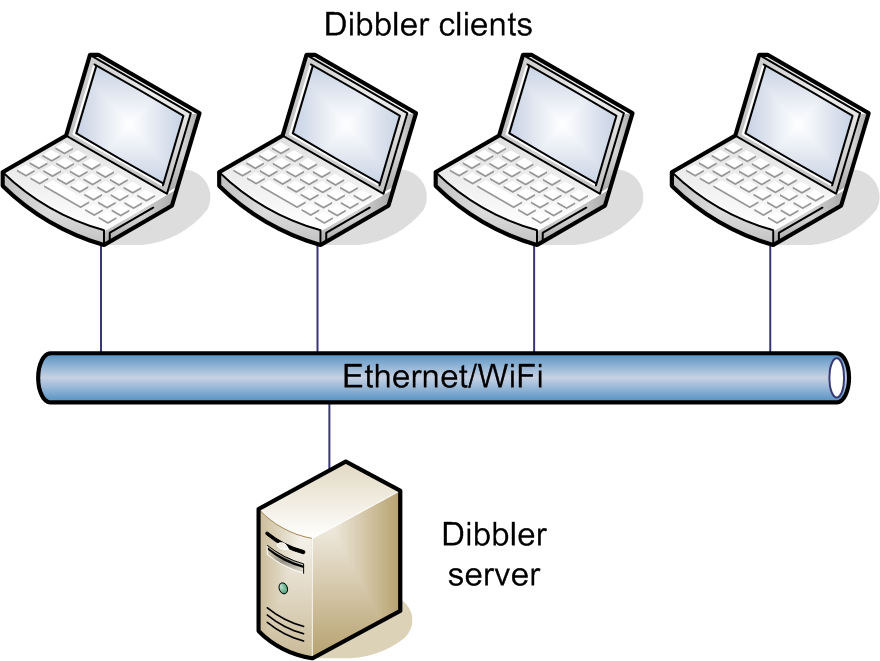
\includegraphics[width=0.6\textwidth]{dibbler-multiple-cli}
\caption{\emph{Several clients supported by one server}}
\end{center}
\end{figure}

\item Server redundancy/Best server discovery -- when client detects
      more than one server available (by receiving more than one
      \msg{ADVERTISE} message), it chooses the best one and remembers
      remaining ones as a backup.

\begin{figure}[ht]
\begin{center}
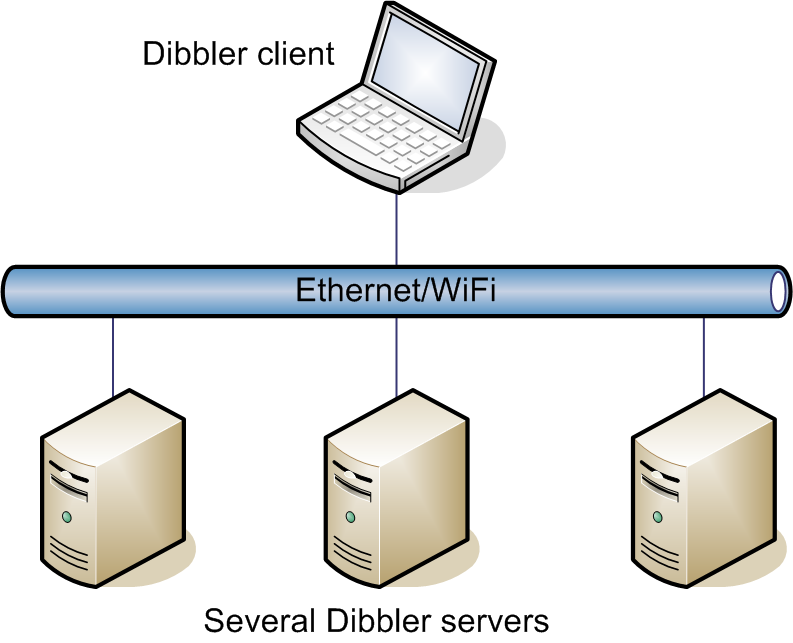
\includegraphics[width=0.6\textwidth]{dibbler-multiple-srv}
\caption{\emph{Redundancy: several servers}}
\end{center}
\end{figure}

\item Multiple servers support -- Client is capable of discovering and
  maintaning communication with several servers. For example, client
  would like to have 5 addresses configured. Prefered server can only
  lease 3, so client send request for remaining 2 addresses to one of
  the remaining servers.
\item Relay support -- In a larger network, which contains several
  Ethernet segments and/or wireless areas, sometimes centrally located
  DHCPv6 server might not be directly reachable. In such cace,
  additional proxies, so called relays, might be deployed to relay
  communication between clients and a remote server. Dibbler server
  supports indirect communication with clients via
  relays. Stand-alone, lightweight relay implementation is also
  available. Clients are capable of talking to the server directly or
  via relays.
\item Address renewal -- After receiving address from a server, client
  might be instructed to renew its address at regular
  intervals. Client periodically sends \msg{RENEW} messege to a
  server, which granted its address. In case of communication failure,
  client is also able to attempt emergency address renewal (i.e. it
  sends \msg{REBIND} message to any server).
\item Unicast communication -- if specific conditions are met, client
  could send messages directly to a server's unicast address, so
  additional servers does not need to process those messages. It also
  improves effciency, as all nodes present in LAN segment receive
  multicast packets.\footnote{Nodes, which do not belong to specific
    multicast group, drop those packets silently. However, determining
    if host belongs or not to a group must be performed on each
    node. Also using multicast communication increases the network
    load.}
\item Duplicate address detection -- Client is able to detect and
  properly handle faulty situation, when server grants an address
  which is illegaly used by some other host. It will inform server of
  such circumstances (using \msg{DECLINE} message), and request
  another address. Server will mark this address as used by unknown
  host, and will assign another address to a client.
\item Power failure/crash support -- After client recovers from a
  crash or a power failure, it still can have valid addresses
  assigned. In such circumstances, client uses \msg{CONFIRM} message,
  to config if those addresses are still valid.
\item Link change detection -- Client can be instructed to monitor its
      link state. Once it detects
\item Normal and temporary addresses -- Depending on its purpose,
      client can be configured to ask for normal (\opt{IA\_NA} option)
      or temporary (\opt{IA\_TA} option). Although use of temporary
      addresses is rather uncommon, both dibbler server and client
      support it.
\item Hint system -- Client can be configured to send various parameters
      and addresses in the \msg{REQUEST} message. It will be treated as
      a hint by the server. If such hint is valid, it will be granted
      for this client.
\item Server caching -- Server can cache granted addresses, so the same
      client will receive the same address each time it asks. Size of
      this cache can be configured.
\item Stateless mode -- Client can be configured to not ask for any
      addresses, but the configuration options only. In such case, when
      no addresses are granted, such configuration is called stateless
      (\msg{INFORMATION-REQUEST} message is used instead of normal
      \msg{REQUEST}).
\item Rapid Commit -- Sometimes it is desirable to quicken configuration
      process. If both client and server are configured to use rapid
      commit, address assignment procedure can be shortened to 2
      messages, instead of usual 4. Major advantage is lesser network
      usage and quicker client startup time.
\item M,O bits from Router Advertisement -- the client can be told to
  observe M(managed) and O(OtherConf) bits from RA and act according
  to them
\item Reconfigure -- server can inform clients that the configuration
  has changed and clients can initiate Reconfigure
\item Authentication: Reconfigure-key -- the server can generate HMAC-MD5
  reconfigure keys on the fly to later authenticate reconfigure
  messages. Clients are able to receive, store and later validate
  against that received key.
\item Authentication: Delayed authorization -- server and client can
  protect their communication against tampering by using
  preprovisioned keys.
\end{itemize}

\subsection{Supported parameters}
Except RFC3315-specified behavior \cite{rfc3315}, Dibbler also supports
several enhancements:

\begin{itemize}
\item DNS Servers -- During normal operation, almost all hosts require
      constant use of the DNS servers. It is necessary for event basic
      operations, like web surfing. DHCPv6 client can ask for
      information about DNS servers and DHCPv6 server will provide
      necessary information. \cite{rfc3646}
\item Domain Name -- Client might be interested in obtaining information
      about its domain. Properly configured domain allow reference to a
      different hosts in the same domain using hostname only, not the
      full domain name, e.g. alice.example.com with properly configured
      domain can refer to another host in the same domain by using 'bob'
      only, instead of full name bob.example.com. \cite{rfc3646}
\item NTP Servers -- To prevent clock misconfiguration and drift, NTP
      protocol \cite{rfc2030} can be used to synchronize clocks. However, to
      successful use it, location of near NTP servers must be
      known. Dibbler is able to configure this information. \cite{rfc4075}
\item Time Zone -- To avoid time-related ambiguation, each host should
      have timezone set properly. Dibbler is able to pass this parameter
      to all clients, who request it. \cite{draft-timezone}
\item SIP Servers -- Session Initiation Protocol (SIP) \cite{rfc3263} is
      commonly used in VoIP solutions. One of the necessary information
      is SIP server addresses. This information can be passed to
      the clients. \cite{rfc3319}
\item SIP Domain Name -- SIP domain name is another important parameter
      of the VoIP capable nodes. This parameter can be passed to all
      clients, who ask for it. \cite{rfc3319}
\item NIS, NIS+ Server -- Network Information Service is a protocol for
      sharing authentication parameters between multiple Unix or Linux
      nodes. Both NIS and NIS+ server adresses can be passed to the
      clients. \cite{rfc3898}
\item NIS, NIS+ Domain Name -- NIS or NIS+ domain name is another necessary
      parameter for NIS or NIS+. It can be obtained from the DHCPv6
      server to all clients, who require it. \cite{rfc3898}
\item Option Renewal Mechanism (Lifetime option)-- All of the options
      mentioned on this list can be refreshed periodically. This might
      be handy if one of those parameters change. \cite{rfc4242}
\item Dynamic DNS Updates -- Server can assign a fully qualified
      domain name for a client. To make such name useful, DNS servers
      must be informed that such name is bound to a specific IPv6
      address. This procedure is called DNS Update. There are two kinds
      of the DNS Updates: forward and reverse. First is used to
      translate domain name to an address. The second one is used to
      obtain full domain name of a known address. See section
      \ref{feature-dns-update} for details. \cite{rfc4704}
\item Prefix Delegation -- Server can be configured to manage a prefix
      pool, i.e. clients will be assigned whole pools instead on
      single addresses. This is very useful, when clients are not
      simple end users (e.g. desktop computers or laptops), but rather
      are routers (e.g. cable modems). This functionality is often
      used for remote configuration of IPv6 routers. \cite{rfc3633}
\end{itemize}

\subsection{Not supported features}
Although list of the supported features increases with each release,
there are certain limitations. Below is a list of such
features:

\begin{itemize}
\item DNS Updates are done over IPv6 only. Adding IPv4 support is
   not planned. Do not bother to develop patches -- Dibbler is a
   IPv6-focused software and IPv4-related patches will be rejected.
\item Conflict resolution in DNS Updates is not supported.
\end{itemize}

\subsection{Operating System Requirements}
\label{requirements}
Dibbler can be run on Linux systems with kernels from 2.4 or later
series. IPv6 (compiled into kernel or as module) support is necessary
to run dibbler. DHCPv6 uses UDP ports below 1024, so root privileges
are required. They're also required to add, modify and delete various
system parameters, e.g. IPv6 addresses.

Dibbler also runs on any Windows systems from Windows XP (Service Pack
1 or later) to Windows 8. Support for Windows 8 has been added in
0.8.3. To install various Dibbler parts (server, client or relay) as
services, administrator privileges might be required. Support for
Windows NT4 and 2000 is limited and considered experimental. Due to
lack of support and any kind of informations from Microsoft, this will
not change. In fact, support for NT4 and 2000 is expected to be
dropped soon. Please post to Dibbler mailing list if you need them.

There is working Mac OS X port available.

Support for FreeBSD, NetBSD and OpenBSD was added in 0.8.1RC1, but
those versions are not very well tested. Support for Solaris 11 has
been added in 0.8.3, but it is still highly experimental. Sources are
confirmed to compile and be able to start operation. Author was not
able to test them thoroughly, so reports regarding confirming their
stability or any discovered issues are welcome. Please report them on
the mailing list. See section \ref{mailing-list}.

See RELEASE-NOTES for details about version-specific upgrades, fixes
and features.

\subsection{Supported platforms}
Although Dibbler was developed on the i386 architecture, there are
ports available for other architectures: IA64, AMD64, PowerPC, HPPA,
Sparc, MIPS, S/390, Alpha and ARMv5. They are available in the PLD,
Gentoo and Debian Linux distributions. Other platforms are likely to
be supported. Keep in mind that author has not tested those ports
himself and need to rely on users' reports, so there might be some
unknown issues present. If this is the case, be sure to notify package
maintainers and possibly the author.

If your system is not on the list, don't despair. Dibbler is fully
portable. Core logic is system independent and coded in C++
language. There are also several low-level functions, which are system
specific. They're used for adding addresses, retrieving information about
interfaces, setting DNS servers and so on. Porting Dibbler to other
systems (and even other architectures) would require implementic only
those serveral system-specific functions. See Developer's Guide for
details.
